% Z-UO-BOOK -- The Triangular Lattice and Universal Optimality (student textbook)
% English translation of papers/discovery_journal_2026/chapters/c08.tex
% Sources: TOP20.json pick 8; papers/textbook_universal_optimality/{publication_meta.json,FACTS.md,editors_note.tex,
%          preface.tex}; results/discovery/D4/verification.md
% Figure: code/fig08.py -> figures/c08_disques.{pdf,png}
\chapter[A textbook, one theorem]{A textbook that follows a theorem all the way to the laboratory}
\reference{Published on 11 October 2026.\\ doi:10.5281/\\zenodo.23295142}

\section*{The idea in one picture}

\begin{analogie}
Think of a rather special cookbook. Each recipe appears in it three times: a step-by-step explanation (why it
works), a laboratory analysis that checks every ingredient and every gesture, and a tasting. Here the ``recipe'' is
a theorem: the explanation is a proof written for a human, the laboratory analysis is the statement verified by the
Lean software, and the tasting is a numerical test in Python and Rust.

\emph{Where the picture stops being accurate:} the analysis checks the recipe against \emph{its own definitions},
not that it produces the dish we wanted; the tasting only says ``nothing looks wrong in the trials made''; and the
main ingredient comes from another kitchen, with no peer review.
\end{analogie}

\section*{What was done}

This 105-page textbook, intended for students, follows a single statement from its definitions to the laboratory:
among all the ways of spreading points in the plane with a given density, the arrangement in triangles (that of the
cells of a beehive, seen through their centres) has the lowest energy, for a whole family of repulsions called
``completely monotone'' (they decrease with distance in a very regular way). This theorem comes from the public
repository openai/math; it was produced by an AI and checked by the Lean kernel. The textbook also teaches everything
needed to understand it: lattices, Poisson summation, theta functions, then the physics where it appears, from
point vortices in fluid mechanics to the vortex lattices of a condensate, to colloids, dusty plasmas and electrons
on helium. A last chapter lists the open questions and student projects.

The five chapters were each written by a separate agent, from one and the same imposed fact sheet, then assembled.
The first rereads an earlier draft and corrects eight errors in it, for example a mix-up between ``derivatives of
strictly alternating signs'' and the true definition, which allows equality.

\paragraph{The book's new result.} To speak of density in an infinite cloud, we count the points in a disc of radius
$R$ and divide by the area $\pi R^2$. Should the points lying \emph{on} the edge be counted? The book proves,
checked by the kernel, that this changes neither the limiting density, nor the energy, nor the conclusion of the
theorem.

\begin{encadre}
\textbf{To do with a pencil.} In the triangular lattice of density one, each point has six nearest neighbours, at
distance $a=\sqrt{2/\sqrt3}\approx1.0746$ (in the book's coordinates, these are the six pairs $(j,k)$ with
$j^2+jk+k^2=1$: $(1,0)$, $(0,1)$, $(-1,0)$, $(0,-1)$, $(1,-1)$, $(-1,1)$). Take a disc centred on a point, of
radius exactly~$a$, of area $\pi a^2=2\pi/\sqrt3\approx3.63$.
\begin{itemize}
\item \emph{Closed} disc (edge included): the centre and its six neighbours, that is $7$ points; $7/3.63\approx1.93$.
\item \emph{Open} disc (edge excluded): the centre alone, that is $1$ point; $1/3.63\approx0.28$.
\end{itemize}
For a small disc, the difference is enormous. But as $R$ grows, the edge weighs nothing against the interior, and
both ratios tend to $1$ (figure~\ref{fig:c08}, left). The theorem turns this intuition into a proof.
\end{encadre}

\begin{figure}[htbp]
\centering
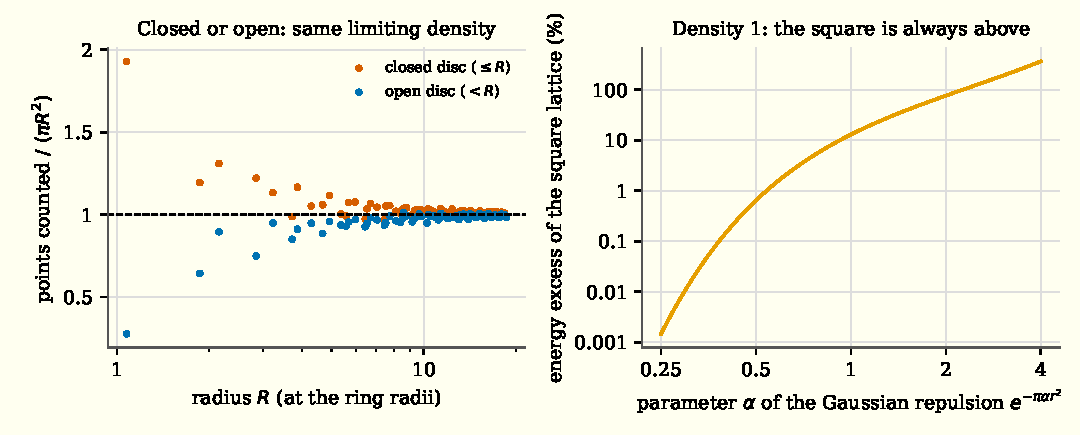
\includegraphics[width=\linewidth]{figures/c08_disques}
\caption{Density counted in a closed or open disc (left); energy excess of the square lattice for a Gaussian
repulsion (right, \niveau{X}).}
\label{fig:c08}
\end{figure}

\section*{How we made sure it is not wrong}

In short: \niveau{A} for the book's new result (open or closed discs), at density one; \niveau{C} at other
densities; the starting theorem is AI-generated and has not been peer reviewed.

For the result on discs, ``the judge has looked'': the Lean kernel, this small program that checks every logical
step, accepted it, with only three standard axioms. The statement was announced before the proof was written. A
separate checker, a distinct AI agent, recompiled it and planted a false proof, which was caught. It even found
better than expected: one of the hypotheses (the cloud has only finitely many points in each disc) is unnecessary,
and it proved this. It also verified, in the kernel, that the equality is not a sleight of hand of the definitions:
for a single point placed on the circle of radius $1$, the open disc counts $0$ and the closed one $1$. It is the
limits that coincide, not the counts. The complete replay of 26 October 2026 passed these two modules without
error.

The whole book was then audited by another instance of an AI model; no human expert has reread it. This audit gave
20 corrections, all applied, and the scripts rerun gave the same results. While writing it, an error was found in an
earlier article of the project: the simulation cut off the potential at a certain distance, and, for the longest
range studied, this cutoff shifted the energies by about $1.8\times10^{-2}$, more than the gap between the
triangular and square lattices. The gap itself hardly changes, but the simulation was about an approximation that
fell outside the theorem's framework. The book publishes this erratum.

\section*{What this does not say}

\begin{limite}
\begin{itemize}
\item The starting theorem is AI-generated and has not been peer reviewed; the whole book depends on it.
\item The result on discs holds for the quantities of the theorem (centred discs, ``lower'' energy); nothing about
  square windows or real boundary conditions. At densities other than one, it stays at level \niveau{C}.
\item The strong version of the conjecture (potential by potential) and the borderline case $s=2$ of power-law
  potentials remain open, as does uniqueness among periodic configurations; the book says so each time. In
  dimensions 8 and 24, the analogous result is proved in the literature, but not formalized here; in dimension 3,
  no universally optimal arrangement is known.
\item The book has no claims register of its own.
\end{itemize}
\end{limite}

\section*{Going further}

The textbook, its \LaTeX{} sources, its scripts and its Lean files are deposited under
doi:10.5281/\allowbreak zenodo.23295142. A critical reading by students, teachers or curious people is explicitly
invited.
